\documentclass[hidelinks,12pt]{article}
\usepackage{fancyhdr}
\usepackage[round]{natbib}
\usepackage{diagbox} 
\usepackage{multirow}
\usepackage{xcolor}
\usepackage{amsmath}
\usepackage{amssymb}
\usepackage{graphicx}
\usepackage{geometry}
\usepackage{wrapfig}
\usepackage{subcaption}
\usepackage{float}
\usepackage{hyperref}
\geometry{scale = 0.85}
\addtolength{\topmargin}{-2.59448pt}
\setlength{\headheight}{37.59448pt}
\bibliographystyle{plainnat}
\rhead{
\includegraphics[scale=0.3]{logo}}
\begin{document}
\title{CZ2002 LAB 4\\
\large OBJ ORIENTED DES \& PROG\\ SS5 GROUP 6}
\date{}
\author{Zou Zeren U2022422H\\}
\maketitle\thispagestyle{fancy}
\tableofcontents
\newpage

\section{Numbers.java Issue}
\textit{The file Numbers.java (in attachment) reads in an array of integers, invokes the selection sort
algorithm to sort them, and then prints the sorted array. Save Sorting.java and Numbers.java to your
directory. Numbers.java won't compile in its current form. Study it to see if you can figure out why.}
\\ \\ 
Numbers.java have to use functions from the Sorting.java.\\
Int is a primitive type, and therefore cannot implement any interface. That's why int[] cannot be passed to a method that expects Comparable[].
To overcome this error, change intList to be an array of Integer (i.e Integer[]), since Integer implements Comparable.
\section{Numbers.java Errors}
\textit{Try to compile Numbers.java and see what the error message is. The problem involves the difference
between primitive data and objects. Change the program so it will work correctly (note: you don't need
to make many changes - the autoboxing feature of Java 1.5 (or higher) will take care of most
conversions from int to Integer). You are to do research in the internet and understand better
autoboxing. }
\begin{itemize}
    \item[] 
\end{itemize}
\qquad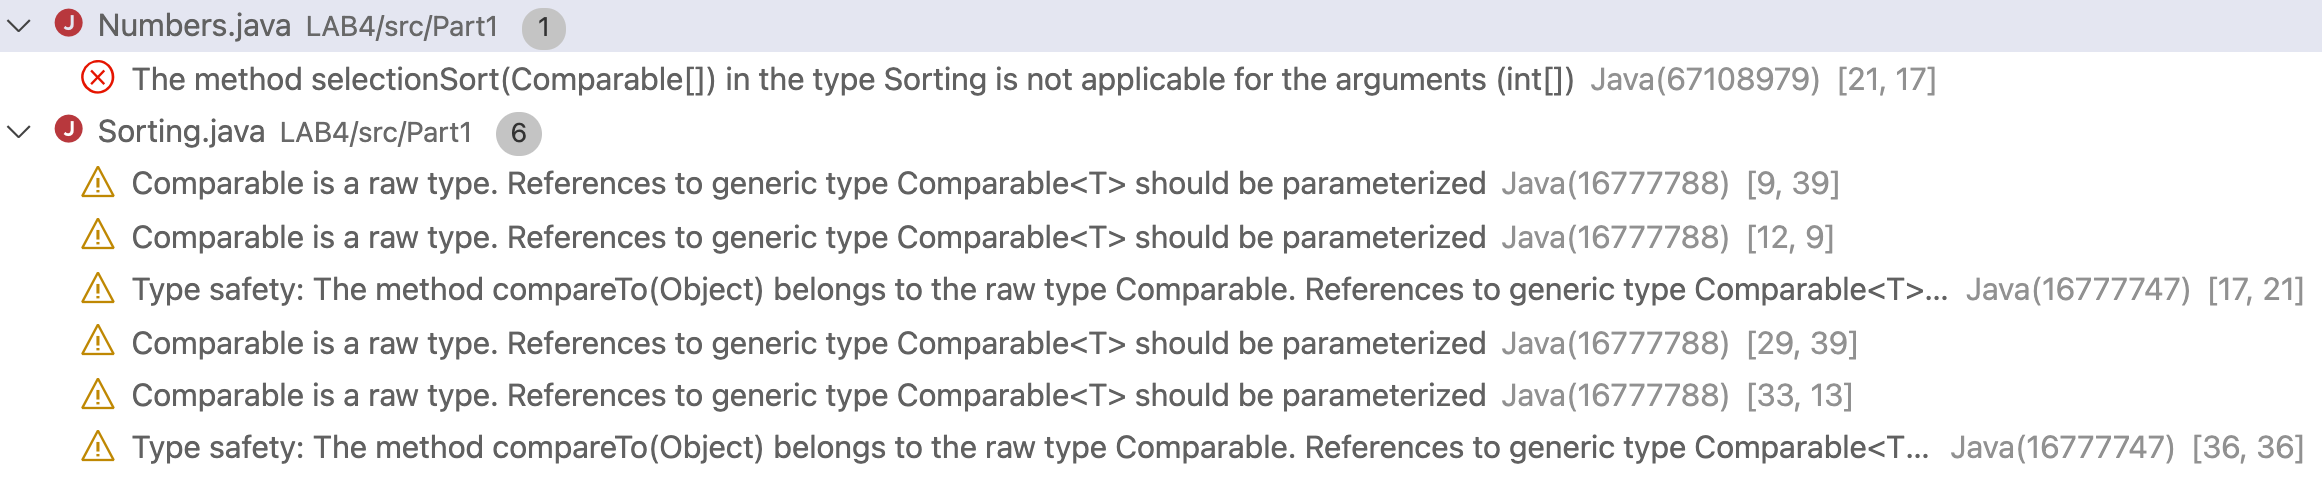
\includegraphics[scale=0.4]{numbers_error.png} 


\begin{itemize}
    \item[] 
\end{itemize}
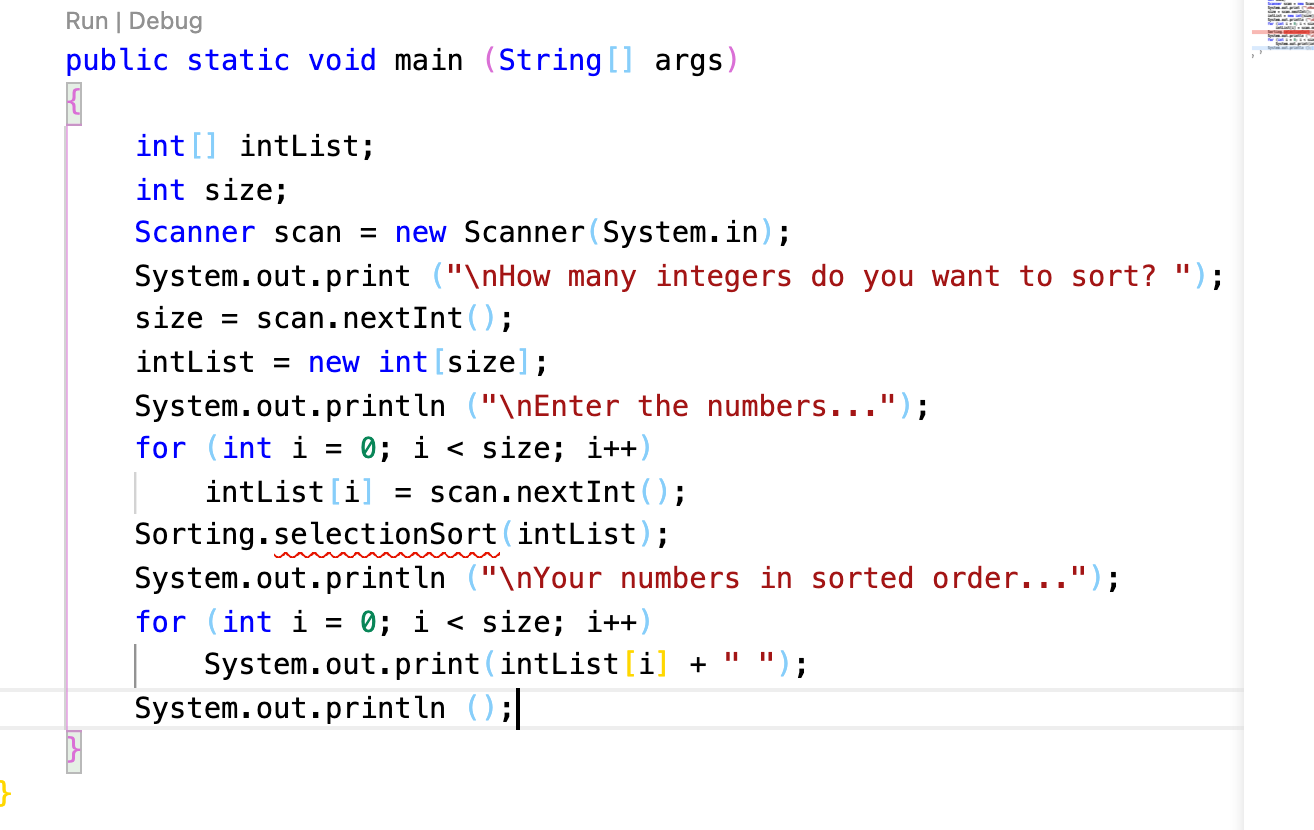
\includegraphics[scale=0.35]{NumbersBef.png}
$\longrightarrow$ 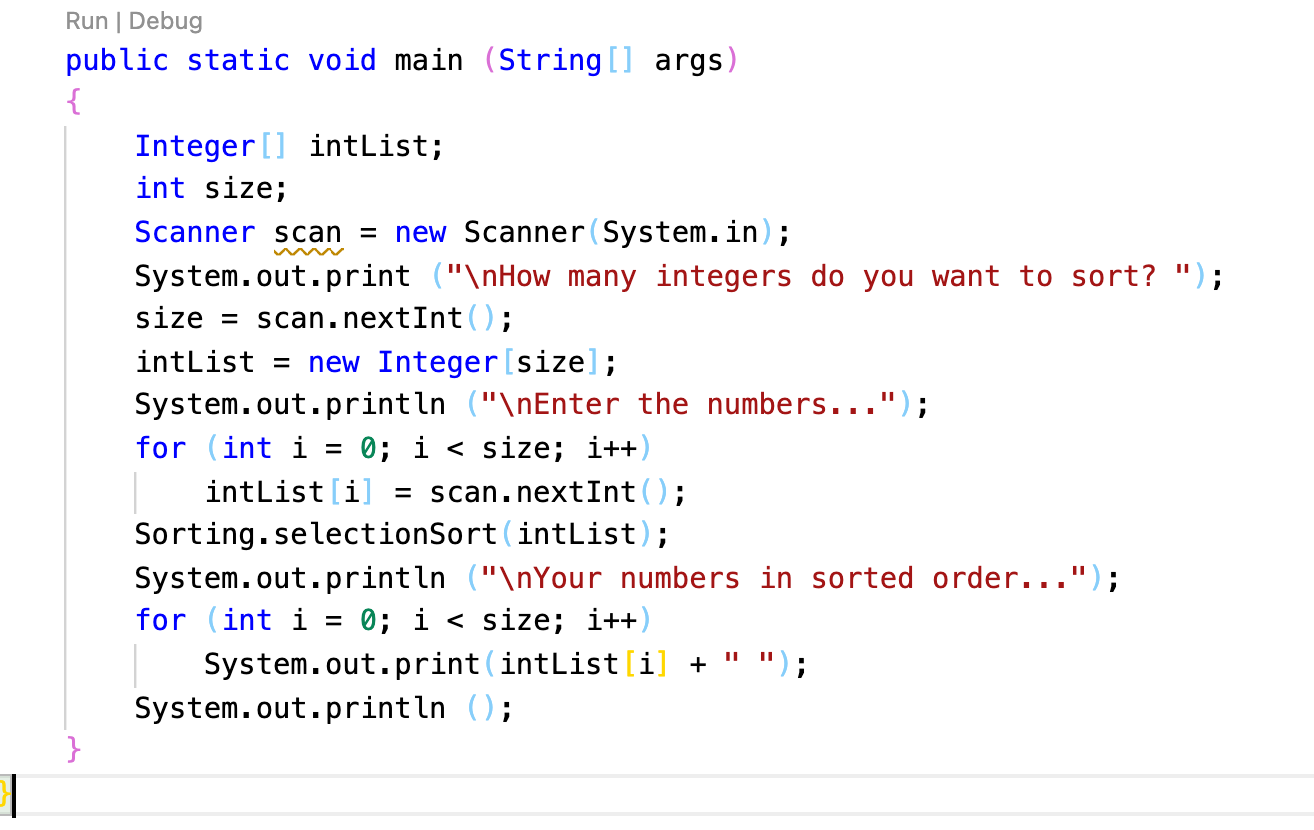
\includegraphics[scale=0.35]{NumbersCode.png}
\\ 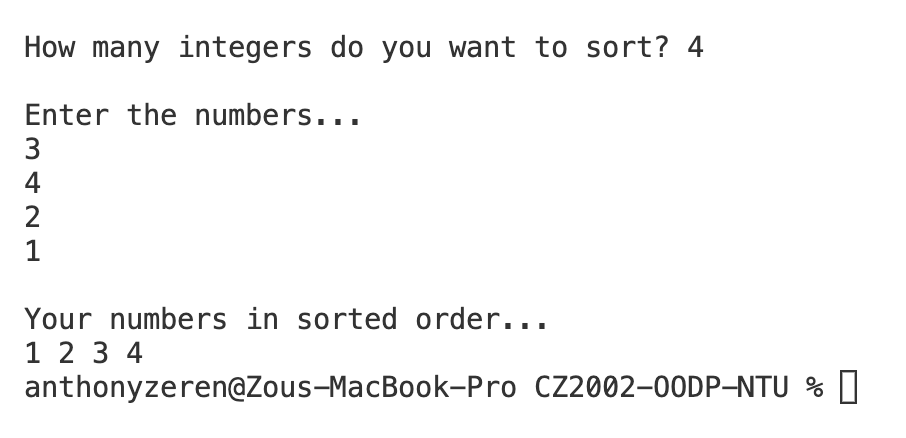
\includegraphics[scale=0.6]{NumbersResult.png}

\section{String.java}
\textit{Write a program Strings.java, similar to Numbers.java, that reads in an array of String objects and sorts
them. You may just copy and edit Numbers.java.}
\begin{itemize}
    \item[] 
\end{itemize}
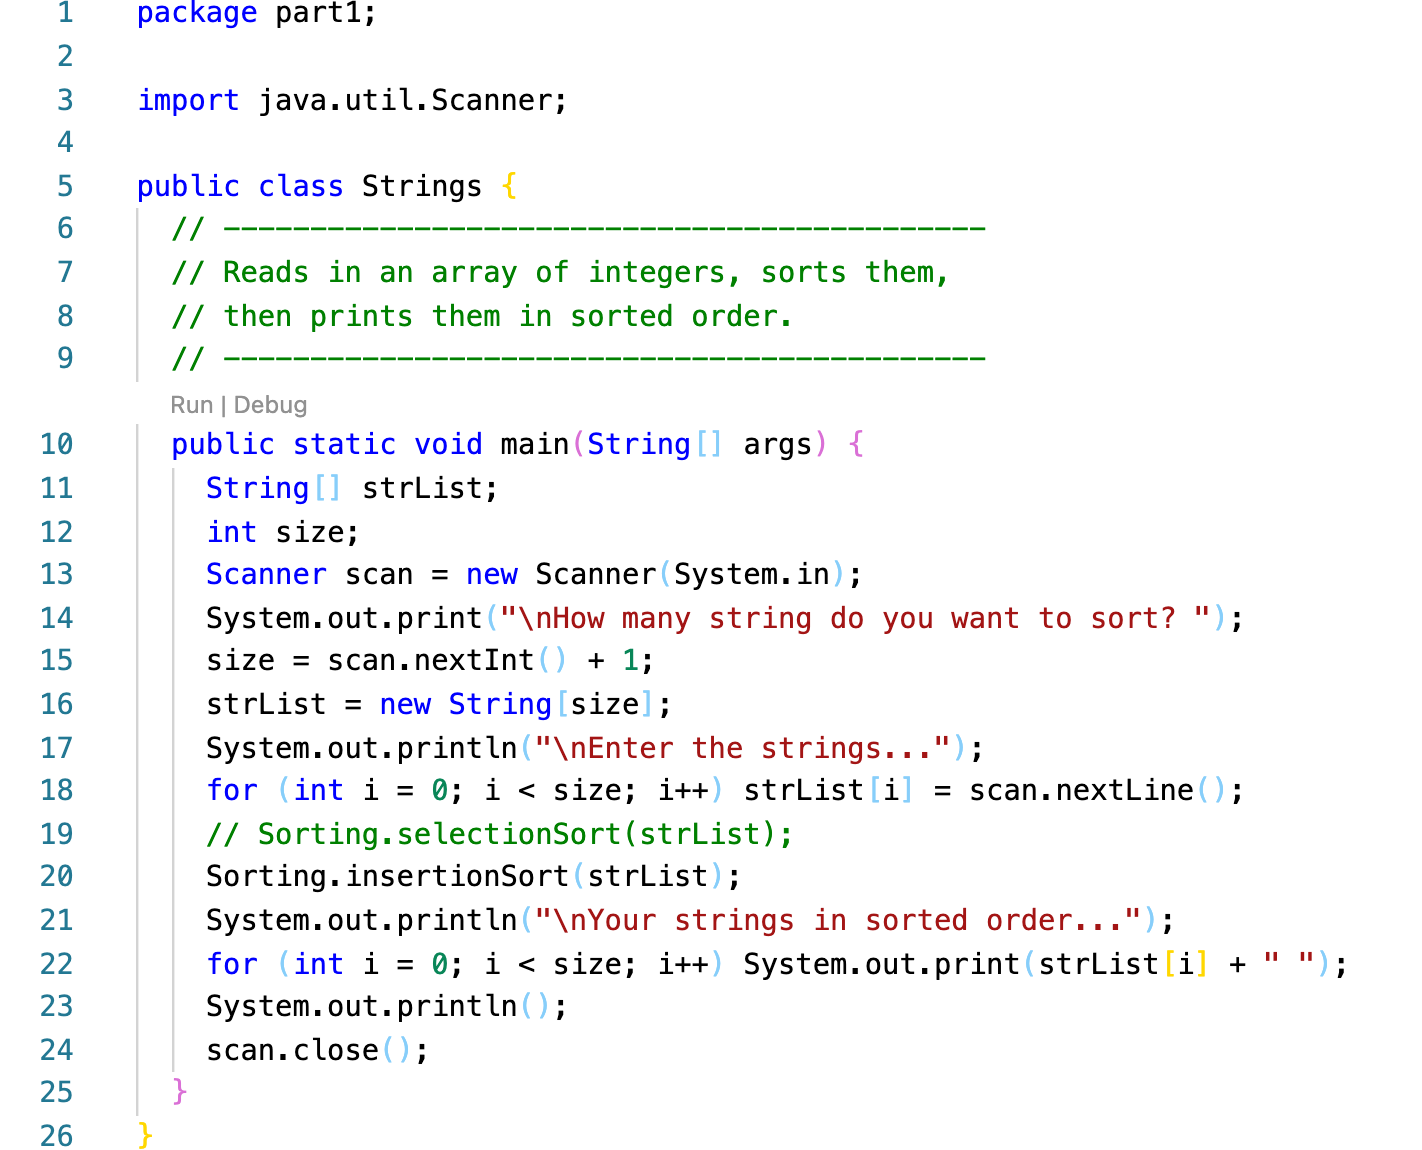
\includegraphics[scale=0.4]{StringCode.png}
$\longrightarrow$ 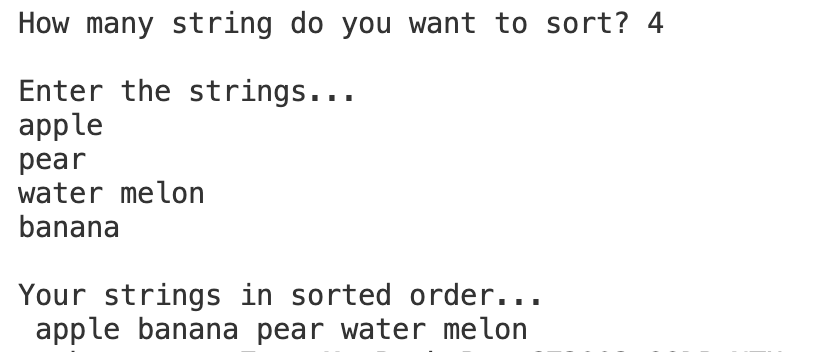
\includegraphics[scale=0.5]{StringsResult.png}
\newpage
\section{Decending Insertion Sort}
\textit{Modify the insertionSort algorithm so that it sorts in descending order rather than ascending order.
Change Numbers.java and Strings.java to call insertionSort rather than selectionSort. Run both to make
sure the sorting is correct.}
\begin{itemize}
    \item[] 
\end{itemize}

Decending Insertion Sort

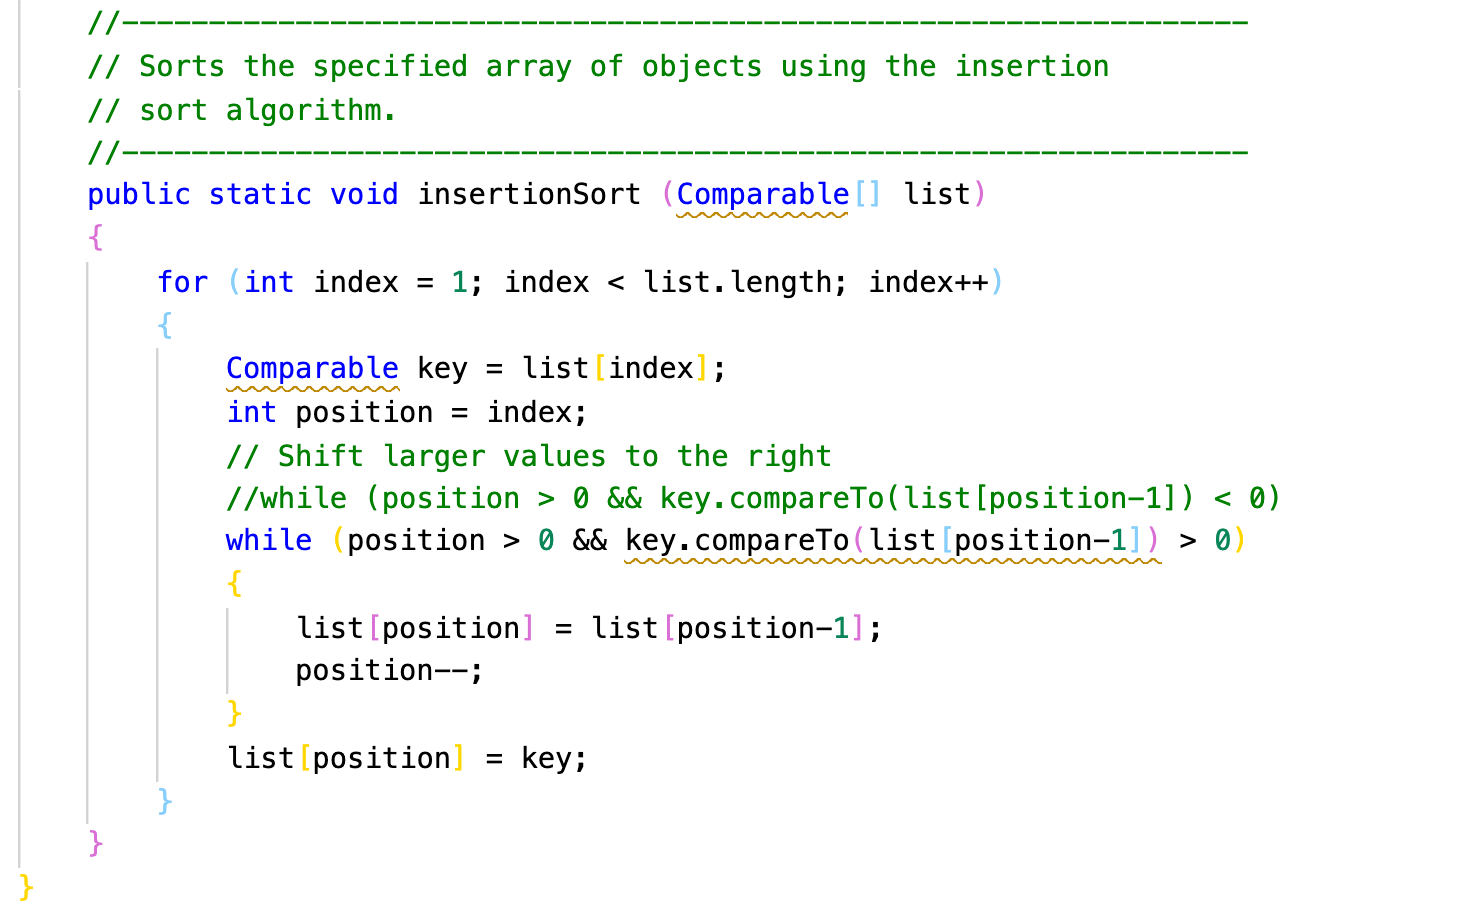
\includegraphics[scale=0.4]{desInsert.png} 

Tested on Numbers

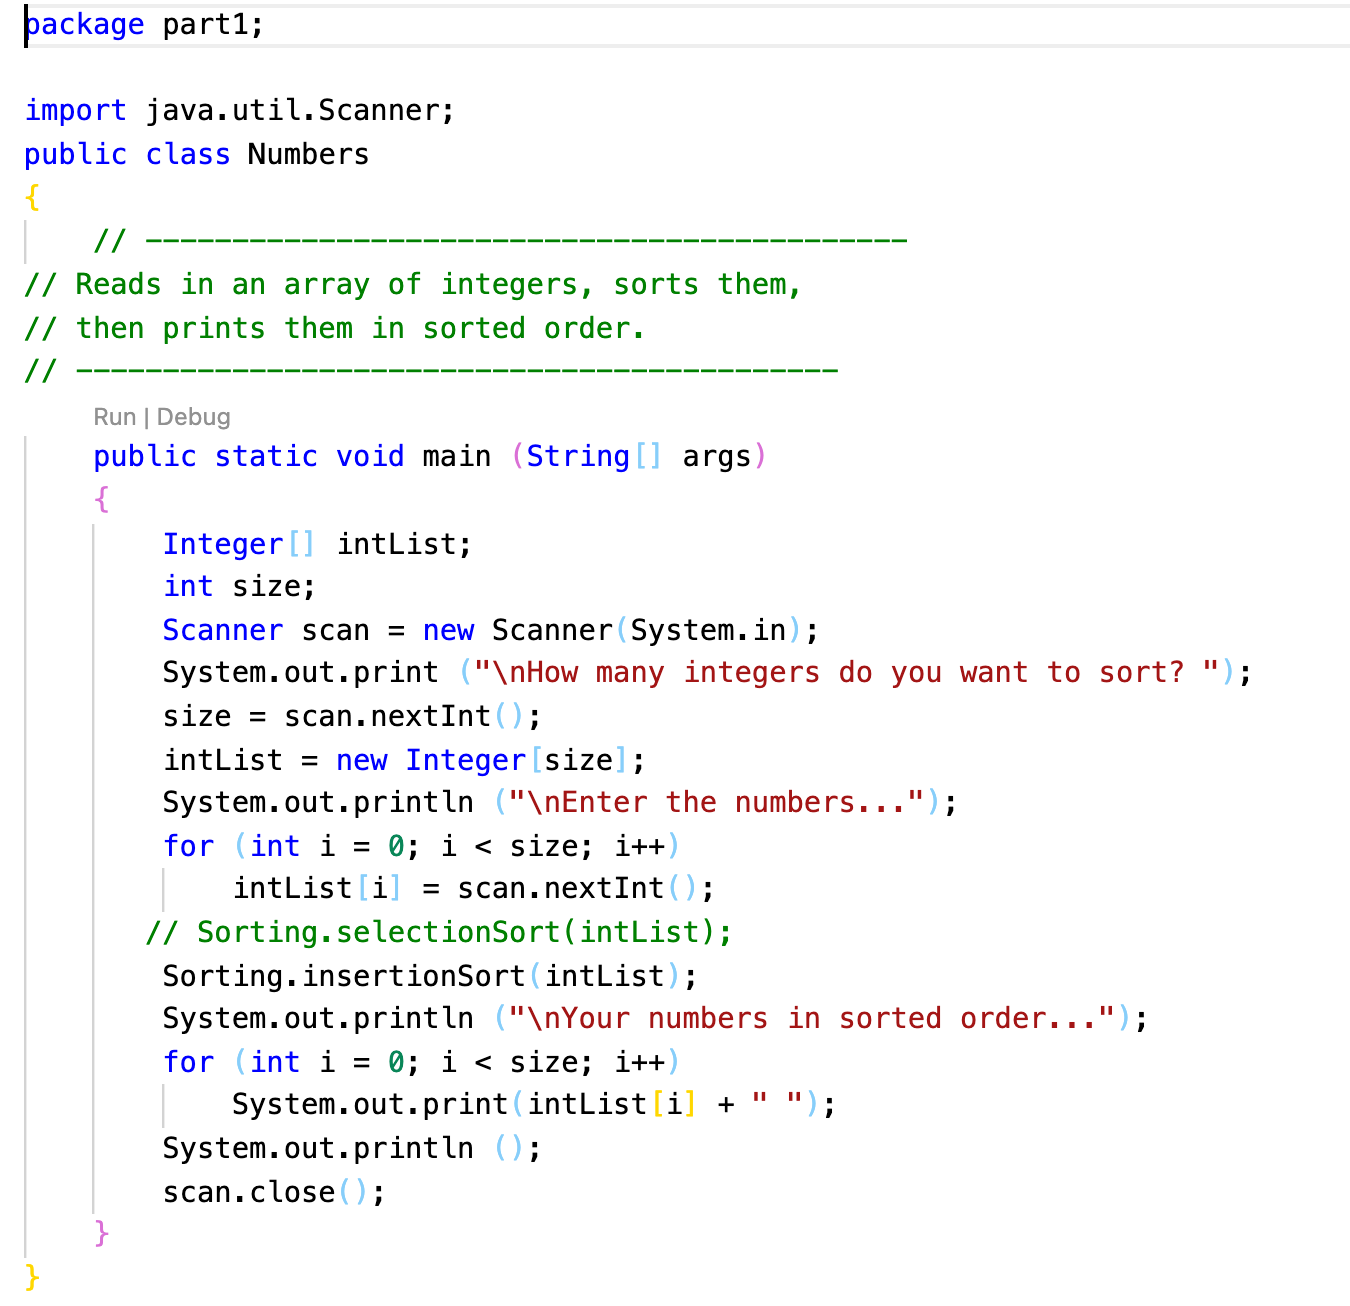
\includegraphics[scale=0.4]{newNum.png}
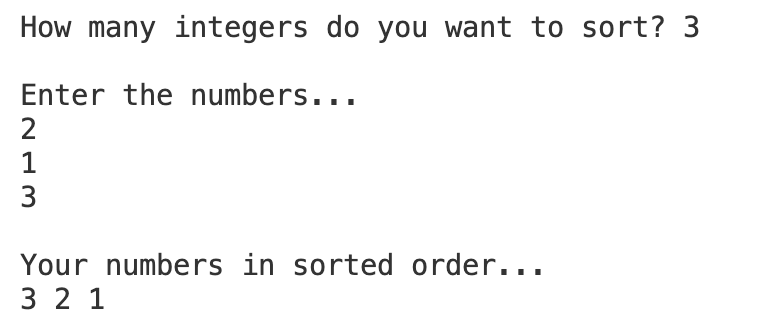
\includegraphics[scale=0.55]{newNumR.png}
\newpage
Tested on Strings

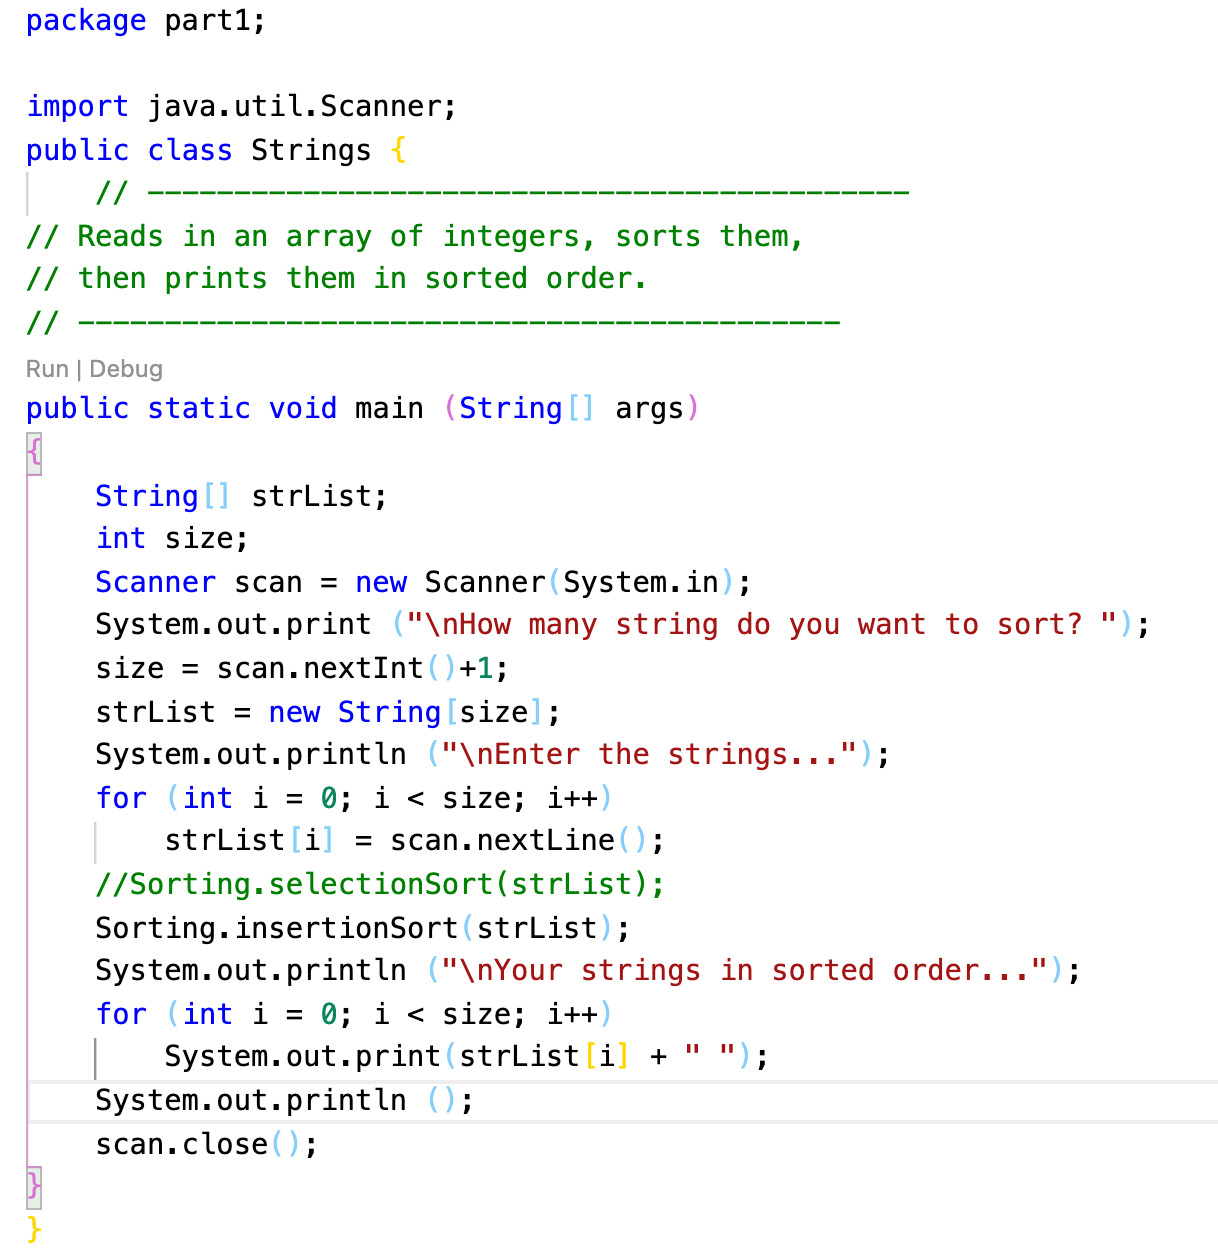
\includegraphics[scale=0.4]{newStrings.png}
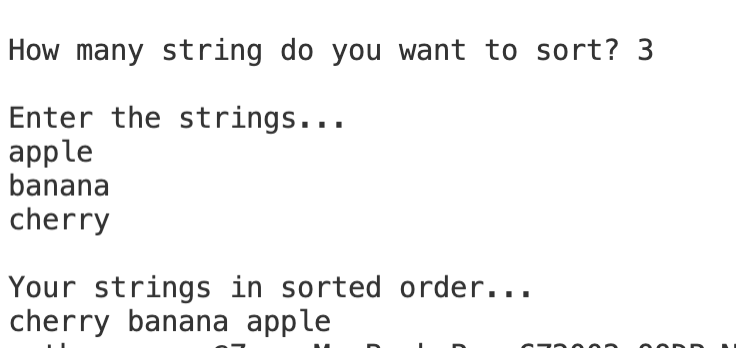
\includegraphics[scale=0.55]{newStringR.png}

\section{SalesPerson Class}
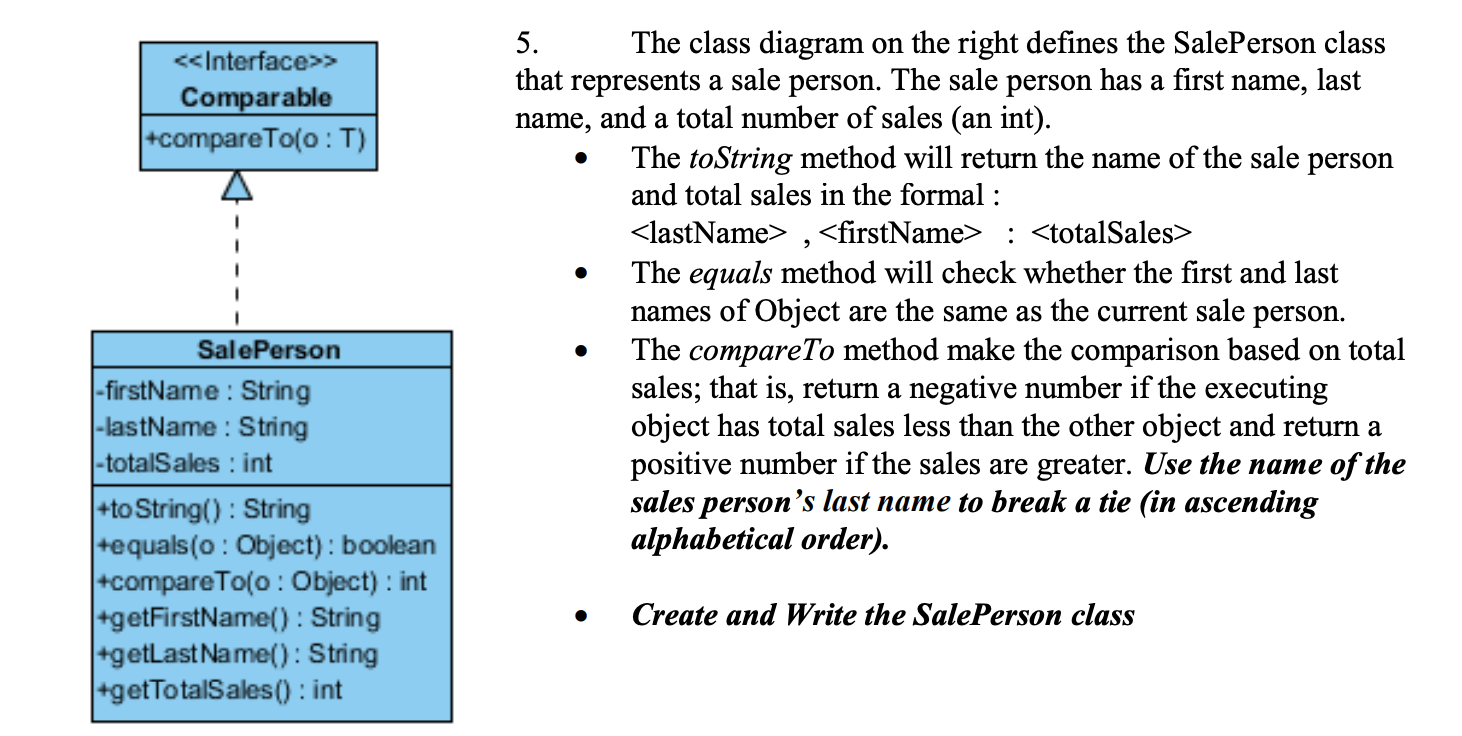
\includegraphics[scale=0.55]{q5.png}
\end{document}